\chapter{Moment Distances from Robust Subspace for Network Anomaly Detection}
\label{ch:4_m_rpca}

\begin{quotation}[]{Paulo Freire}
No one knows it all. No one is ignorant of everything. We all know something. We are all ignorant of something.
\end{quotation}

Some widely adopted algorithms for anomaly detection assume a Gaussian or symmetric distributed data, however this assumption may not be observed in some real world problems, such as the case of network traffic analysis, where network traffic features are usually more characterized by skewed and heavy-tailed distributions \cite{lakhina2005mining,benson2010network, leon2017probability}.

Findings of Benson \emph{et al.}  \cite{benson2010network} indicate that certain positive skewed and heavy-tailed distributions can model data center switch traffic, and highlights a difference between the data center environment and the wide area network, where the long-tailed Pareto distribution typically shows the best fit \cite{benson2010network}. Leon-Garcia \cite{leon2017probability} also argues that Pareto distribution has been found to capture the behavior of many quantities of interest in the study of Internet behavior. Moreover, Benson \emph{et al.}  \cite{benson2010network} observes that the Lognormal distribution is the best fit to model arrival processes in a data center.

These findings show that the skewness and heavy-tailed distributions may be important for network traffic analysis, and can motivate researches to evaluate the impact of skewed data into algorithms that rely on Gaussian distributed data. These findings can also highlight opportunities to  exploit the skewness and heavy-tailed distributions to obtain accurate classifiers for network anomaly detection.

An outlyingness-approach based on a robust estimator of skewness, combined with robust estimators of location and scale, can be able to flag the outlying measurements. When the same methodology would be used with non-robust estimators of location, scale and skewness, the outlyingness-values would be affected by the outliers such that the outlying group could be masked \cite{hubert2009robustskewed}.

Network anomaly detection problems are usually characterized by imbalanced data \cite{Phua2004minority,he2008learning,benson2010network}. However, learning algorithms for imbalanced data has been a challenging research topic, considering that the fundamental issue with the imbalanced learning problem is the ability of imbalanced data to significantly compromise the performance of most standard learning algorithms \cite{he2008learning}. Therefore, learning methods for imbalanced and skewed data have been attracted attention of researchers \cite{Phua2004minority,hubert2009robustskewed}.

We believe that the skewness of anomalous and normal traffic can highlight features for improving anomaly detection in imbalanced data. We also believe that the distance between robust estimates of normal traffic and contaminated observations can highlight discrepancies and be used for network attack detection. 

Therefore, we propose the m-RPCA, which is an approach based on distances between moments computed from a robust subspace learned by Robust Principal Component Analysis (RPCA) and contaminated observations, in order to detect anomalies from skewed data and network traffic. The proposed approach relies on a robust subspace computed from supposed normal observations, for estimating the moments to be used for distance analysis. The anomaly detection from contaminated observations evaluate the Mahalanobis distance between the robust moments and new contaminated observations, in a semi-supervised fashion, without the computational cost of new robust subspace learning for new observations. The m-RPCA can also be computed as an unsupervised algorithm, with subspace learning from the same contaminated data that is the target of the anomaly detection analysis.

We evaluate the accuracy of the m-RPCA for anomaly detection on simulated data sets, with skewed and heavy-tailed distributions, and for the CTU-13 data set \cite{garcia2014empirical}, which is a large data set of normal, background and botnet traffic that has been adopted to deal with the lack of up-to-date real-world data sets for anomaly detection systems \cite{osanaiye2016distributed}. The Experimental evaluation compares our proposal to widely adopted algorithms for anomaly detection based on clustering and statistical approaches. We also compare the results to ROBPCA \cite{hubert2005robpca}, which is a method that also relies on robust estimates with adjusted outlyingness based on robust skewness.

The main contribution of this work is the proposal of a novel semi-supervised and unsupervised method for anomaly detection in skewed and imbalanced data, with results of experimental evaluation on simulated and real data sets.

This Chapter is organized as follows. In Section \ref{sec:4_relatedworks}, it is conducted a literature review of network anomaly detection, botnet detection, and imbalanced learning. Section \ref{sec:4_datamodel} presents the data model and the evaluated data set. Section \ref{sec:4_proposal} describes the proposed approach for network attack detection. Section \ref{sec:4_experiments} discusses the experimental validation, Section \ref{sec:4_simulated_result} presents the results of the simulated scenarios and the Section \ref{sec:4_ctu13_result} describes the results for anomaly detection on CTU-13 data set. Finally, Section \ref{sec:4_conclusion} draws the conclusions and the suggestions for future work.


\section{Related Works}
\label{sec:4_relatedworks}

% network anomaly detection
Network Anomaly detection has emerging as an important approach for securing communication networks and to deal with the increasing number of network attacks. Bhuyan \emph{et al.} \cite{bhuyan2014network} provide an overview of facets of network anomaly detection, present attacks normally encountered by network intrusion detection systems, and categorize existing network anomaly detection methods and systems based on the underlying techniques. Ahmed \emph{et al.} \cite{ahmed2016survey} present an analysis of four major categories of anomaly detection techniques, which include classification, statistical, information theory and clustering. Moustafa \emph{et al.} \cite{moustafa2019holistic} discuss aspects of anomaly-based Network Intrusion Detection Systems (NIDSs), describing details of cyber-attacks and new solutions for anomaly detection, and provides a benchmark data sets for training and validating approaches for network anomaly detection.

% botnet detection
A botnet is a network of bots, that are compromised machines under the influence of malware (bot). The botnet is commandeered by a botmaster and used as resource for attacks, such as distributed denial-of-service (DDoS) attacks, and fraudulent activities such as spam, phishing, identity theft, and information ex-filtration. We refer to \cite{ahmed2016survey} and \cite{moustafa2019holistic} for an overview of network attacks. The botmaster coordinate a botnet through a command and control (C\&C) channel where bots receive commands and synchronize attacks and fraudulent activities. Centralized C\&C structures using the Internet Relay Chat (IRC) protocol have been utilized by botmasters for a long time, but other protocols, such as HTTP, and architectures, such as Peer-To-Peer, have also been adopted \cite{gu2008botminer}.

Acarali \emph{et al.} \cite{acarali2016survey} surveys network-based detection approaches for HTTP-based botnets, and discuss the traffic-based features used to detect bot traffic and presents an abstraction of the main types of features related to protocols and OSI layers. Wang \emph{et al.} \cite{Wang2018ddosbotnetssurvey} present an analysis based on 50,704 different Internet DDoS attacks originated of 674 botnets from 23 different botnet families with a total of 9,026 victim belonging to 1,074 organizations in 186 countries. Their analysis reveals that geolocation of the attacking sources follows patterns and enables source prediction, and highlights that multiple attacks to the same target also exhibit strong patterns of inter-attack time interval, also presents that there is a trend for different botnets to launch DDoS attacks targeting the same victim, simultaneously or in turn.

The BotHunter was proposed by Gu \emph{et al.} \cite{gu2007bothunter} to detect the infection and coordination of botnets by matching sequence model, through a correlation approach for detecting stages of the infection process.  Gu \emph{et al.} \cite{gu2008botminer} presented the BotMiner, which aims to detect groups of compromised machines that are part of a botnet. BotMiner monitors communications that may suggest C\&C or malicious activities, and finds a coordinated group pattern by means of clusters of similar communication activities, clusters of similar malicious activities, and performs cross cluster correlation to identify the hosts that share both similar communication patterns and similar malicious activity patterns.

Khattak \emph{et al.} \cite{khattak2015botflex} proposed BotFlex, which is a network-based tool for botnet detection, composed by a Complex Event Processing (CEP) engine and on a correlation framework that continuously receives events and correlates them according to rules. BotFlex's results are compared to BotHunter \cite{gu2007bothunter}, but the evaluation relies in a own and not public data set.

Several approaches for network attack detection uses the KDD 99 \cite{ahmed2016survey,osanaiye2016distributed,bhuyan2014network} data sets for accuracy and performance evaluation, due to their availability and labeled attacks. Even though the KDD 99 data set are criticized by the generation procedure and the risk of over-estimations of anomaly detection due to data redundancy, it still represents one of the few publicly available labeled data sets currently in use today by researchers \cite{osanaiye2016distributed,bhuyan2014network}. NSL-KDD \cite{tavallaee2009detailed} data set is the refined version of the KDD 99 data set that removed the redundant data records, in order to avoid biased classifications. However, NSL-KDD data set maintain the limitations of the KDD 99 regarding volume and lacks on reproduction of recent network traffic and attacks.

The objective of Garcia \emph{et al.} \cite{garcia2014empirical} is to compare three botnet detection methods by means of a simple and reproducible methodology, by a good data set and by a new error metric. This paper evaluates some data sets for network anomaly detection, and surveys some approaches for botnet detection, and proposes two methods (BClus and CAMNEP) for botnet detection, comparing results to BotHunter \cite{gu2007bothunter}.

Considering the lack of available labeled data sets, Garcia \emph{et al.} \cite{garcia2014empirical} proposes the CTU-13 data set, which is composed by attack, normal and background labeled data, in an imbalanced distribution like in a real networks. The authors recommend scenarios for training and testing in order to avoid the use of traffic from a botnet family for training and testing, aiming to ensure that the evaluated methods can generalize and detect new behaviors. Taking into account the adoption of unsupervised or semi-supervised approaches for anomaly detection, adopting the training and testing approach proposed by Garcia \emph{et al.}, some botnet malwares wouldn't be tested, since in the author's proposal some botnets are present only for training.

Wang and Paschalidis \cite{wang2017botnet} proposed a botnet detection approach based on anomaly and community detection, aiming for detecting botnets and identifying bots before the botnet becomes active. The first stage detects anomalies by leveraging large deviations of an empirical distribution. The second stage detects the bots using ideas from social network community detection in a graph that captures correlations of interactions among nodes over time. This work is compared to the BotHunter \cite{gu2007bothunter} for the CTU-13 botnet data set \cite{garcia2014empirical}.

% Anomaly detection by subspace learning
Traditional PCA-based anomaly detection models are not suitable for anomaly interpretation, as they judge whether a data instance is an anomaly or not based on the length of its projection on the abnormal subspace spanned by the less significant principal components, and there is no direct mapping between PCA’s dimensionality-reduced subspace and the original feature space \cite{ringberg2007sensitivity}. However, to overcome the above mentioned limitations, some approaches based on PCA have been proposed for network anomaly detection. Callegari \emph{et al.} \cite{callegari2011novel} proposed a PCA-based method for identifying the network traffic flows responsible for an anomaly detected at the aggregate level, by means of a separation of normal and anomalies according to principal components (normal) and remaining (anomalies). Lee \emph{et al.} \cite{Lee2013} presented OverSampling PCA (osPCA), which allows one to determine the anomaly of the target instance according to the variation of the resulting dominant eigenvector obtained by similarity analysis and over sampling. Vieira \emph{et al.} \cite{vieira2017model} proposed a framework that applies Model Order Selection (MOS) for detection of time frames under attack and uses similarity analysis to extract details and detect the time and ports under attack.

% Anomaly detection by robust subspace learning
The problem of PCA or subspace learning for outlier corrupted data is called Robust Principal Component Analysis (RPCA) or robust subspace learning \cite{candes2011robust, vaswani2018robust}. RPCA aims to be resilient to outliers by means of a robust subspace learning \cite{vaswani2018robust} for outlier corrupted data, decomposing a given data matrix $\pmb{X}$ into the sum of a low rank matrix $\pmb{L}$, whose column subspace gives the principal components, and a sparse matrix $\pmb{S}$, which refers to outliers’ matrix. This definition is also referred to as the sparse + low rank ($\pmb{S + LR}$) formulation \cite{vaswani2018robust}. We refer to \cite{lerman2018overview} and \cite{vaswani2018robust} for more details regarding robust subspace learning.

RPCA is been mainly applied to computer vision, in problems of robust subspace tracking and robust subspace recovery. However, RPCA has also been adopted for general outlier detection \cite{hubert2005robpca,hubert2009robustskewed,cherapanamjeri2017thresholding,zhou2017anomaly,NetflixSurus} and for anomaly detection on network traffic \cite{pascoal2012robust}. ROBPCA \cite{hubert2005robpca} intends to identify outliers using PCA from robust estimates of mean and covariance matrix, to reduce the data dimensions and plotting the orthogonal distances versus the robust score distances, to flag an outlier map. However, ROBPCA flags many points as outlying when the original data is skewed. Therefore, Hubert \emph{et al.} \cite{hubert2009robustskewed} proposed ROBPCA-AO, which improves ROBPCA for problems with skewed data, by means of an adjusted outlyingness based on robust skewness. Hubert \emph{et al.} \cite{hubert2009robustskewed} evaluated ROBPCA-AO for real and simulated data sets, but it is not clear if this method was evaluated for very skewed and imbalanced data sets, such as in the network attack detection problem.

Robust subspace learning has receiving a growing attention of researchers aiming the development of network anomaly detection systems \cite{rousseeuw1984mcd, rousseeuw1999fastmcd, hubert2005robpca,hubert2009robustskewed, pascoal2012robust, zhou2017anomaly}, considering outlier-robust methods and sparse-corruption methods \cite{lerman2018overview}. Pascoal \emph{et al.} \cite{pascoal2012robust} proposed an approach based on a robust mutual information estimator for feature selection and based on RPCA for outlier detection in internet traffic. The anomaly detection proposed by Pascoal \emph{et al.} is an unsupervised approach that estimate the first $k$ robust principal components, calculate the score and the orthogonal distances, calculate the thresholds and classify new observations accordingly. Zhou and Paffenroth \cite{zhou2017anomaly} proposed the Robust Deep Autoencoders (RDA), which the central idea is that a RDA inherits the non-linear representation capabilities of autoencoders combined with the anomaly detection capabilities of RPCA. Considering that outliers and noise may reduce the quality of representations discovered by deep autoencoders, the proposed model isolates noise and outliers in the input by means of a RPCA approach, and the autoencoder is trained after this isolation. RDA was evaluated by the authors for the MNIST data set.

Benson \emph{et al.} \cite{benson2010network} conducted an empirical study of the network traffic in 10 data centers belonging to three different types of organizations, including university, enterprise, and cloud data centers. Findings of Benson \emph{et al.} indicate that certain positive skewed and heavy-tailed distributions can model data center switch traffic, and highlights a difference between the data center environment and the wide area network, where the long-tailed Pareto distribution typically shows the best fit \cite{benson2010network}.

Mahalanobis Distance (MD) is a generalized distance which is useful for determining the similarity between an unknown sample and a collection of known samples, by considering the covariance between the variables and their mean values. The MD is a measure of the distance between a vector $\pmb{x}$ and a distribution $\pmb{X}$, introduced by P. C. Mahalanobis in 1936 \cite{mahalanobis1936md}. It is a multi-dimensional generalization for measuring how many standard deviations away $\pmb{x}$ is from the mean $\bar{\pmb{x}}$ and covariance $\bar{\pmb{\Sigma}}$ of $\pmb{X}$. MD has been used for distance based anomaly detection with robust estimates in many areas, assuming that the Mahalanobis Distance between robust estimates and contaminated observations can reveal anomalies.

We propose an approach based on the distances between moments computed from learned robust subspace and contaminated observations, for anomaly detection on skewed and imbalanced data sets, and evaluate our approach for network attack detection. The proposed approach relies on learning robust subspace from supposed normal traffic for estimating the moments (mean, skewness and kurtosis). Thus, the anomaly detection for contaminated observations should evaluate the Mahalanobis Distance between the robust moments and contaminated observations, in a semi-supervised fashion and without the computational cost of new robust subspace learning for new observations, or in a unsupervised approach, where the robust subspace is learned from the contaminated data and the distance analysis is between the robust moments and the contaminated observations. 


\section{Data Model}
\label{sec:4_datamodel}

In this paper, scalars are denoted by italic letters (\emph{a, b, A, B, $\alpha$, $\beta$}), vectors by lowercase bold letters ($\pmb{a}, \pmb{b}$), matrices by uppercase bold letters ($\pmb{A}$, $\pmb{B}$), and $a_i,_j$ denotes the (\emph{i, j}) elements of the matrix $\pmb{A}$. The superscripts \textsuperscript{T} and \textsuperscript{-1} are used for matrix transposition and matrix inversion, respectively. The Frobenius norm is denoted as $\left\| \mathord{\cdot} \right\|_F$, while $\left\| \mathord{\cdot} \right\|_*$ denotes the nuclear norm of a matrix and $\left\| \mathord{\cdot} \right\|_1$ means the sum of the absolute values of matrix entries. We also define the operator $\langle \mathord{\cdot} \rangle$, that is the standard trace inner product, and $[ \mathord{\cdot} ]^s$, which denotes the $n$ largest values of a vector.

This section also presents a description of the simulated data model in Subsection \ref{sec:4_simulation} and in Subsection \ref{sec:4_CTU-13} we describe the data model for the CTU-13 data set.


\subsection{The Simulated data set}
\label{sec:4_simulation}

In order to analyse the null hypotheses $H_{1rob.sub}$ and $H_{0rob.sub}$, which evaluate if the robust subspace learning can improves the anomaly detection from imbalanced and skewed data, we create two simulated data sets characterized by skewed and heavy tailed distributions, and create a simulated Gaussian distributed data set, in order to also analyse the detection rate for not skewed and not heavy tailed distributions.

We selected Pareto (with scale $a=3$, mode $m=1$ and $\mu=1$) and Lognormal (with mean $\mu=0$ and standard deviation $\sigma=1$) distributions, denoted respectively as $\pmb{Y}_p$, while $\pmb{Y}_l$, to simulate normal events and to evaluate the anomaly detection on skewed data performed by our proposals in comparison to widely adopted algorithms for outlier detection, considering that these distributions are skewed and heavy-tailed, and have been adopted to characterize network traffic of the Internet and data centers \cite{benson2010network,leon2017probability}. We also adopt the Gaussian distributed data set $\pmb{Y}_g$ to simulate normal events with mean $\mu=0$ and unitary standard deviation $\sigma=1$.

The addictive anomalies for Pareto and Lognormal distributions are white Gaussian noise with mean $\mu=0$ and unitary standard deviation $\sigma=1$. The Pareto distribution contaminated by Gaussian noise is denoted as $\pmb{Y}_p^c$, while $\pmb{Y}_l^c$ denotes the Lognormal distribution contaminated by Gaussian noise. The $\pmb{Y}_p^c$ and $\pmb{Y}_l^c$ are depicted by the Figures \ref{fig:4.01} and \ref{fig:4.02}, in order to provide a visual example one variable of $\pmb{Y}_p^c$ and $\pmb{Y}_l^c$.

\begin{figure}[!htb]
	\centering
	\subfigure[Pareto and Gaussian Anomalies]{%
		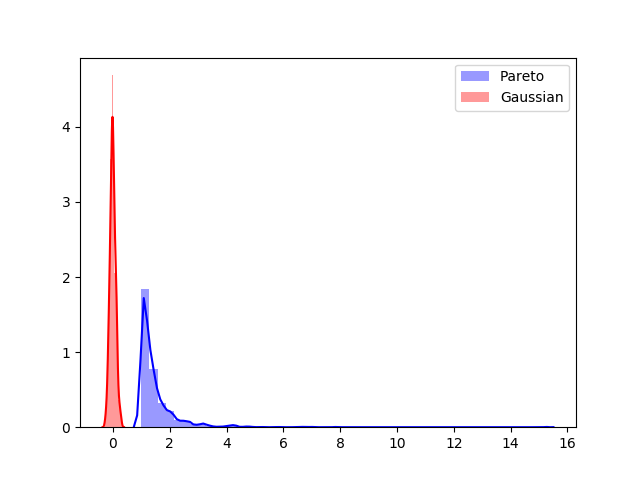
\includegraphics[width=0.48\textwidth]{figures/ch4/4_Xpg2.png}
		\label{fig:4.01}
	}
	\subfigure[Lognormal and Gaussian Anomalies]{%
		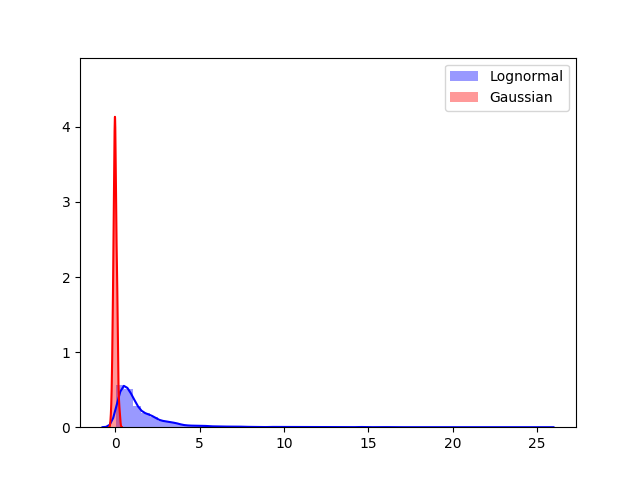
\includegraphics[width=0.48\textwidth]{figures/ch4/4_Xlogng2.png}
		\label{fig:4.02}
	}
	\caption[Examples of skewed and heavy tailed distributions]{Examples of skewed and heavy tailed distributions}
	\label{fig:4.03}
\end{figure}

An uniform noise between $-6$ and $6$ is used to add anomalies into the Gaussian distributed data set, and $\pmb{Y}_g^c$ denotes the contaminated Gaussian data contaminated by an uniform distribution. The figure \ref{fig:4.04} shows an example of the Gaussian distribution of normal observations and the uniform distribution to simulate the addition of anomalies.

\begin{figure}[h!]
	\centering
	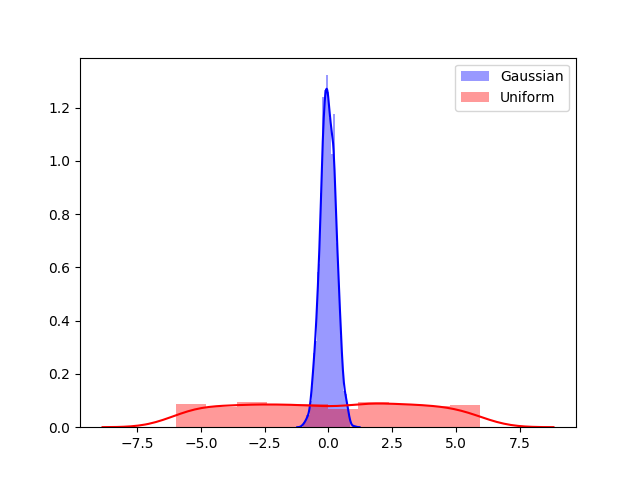
\includegraphics[width=8cm]{figures/ch4/4_Xgu2.png}
	\caption{Example of Gaussian and Uniform Anomalies}
	\label{fig:4.04}
\end{figure}

Each contaminated data set is composed by a number of legitimate observations and contaminated samples. We evaluate contamination rates $c$ between 1\% and 50\%, to simulate the imbalanced data of anomaly detection problems during our experiments. This data sets simulate a total of 2400 events for each scenario with contaminated Pareto, Lognormal and Gaussian. Therefore, the number of legitimate observations is defined according to the contamination rate selected for each evaluation.


\subsection{The CTU-13 data set}
\label{sec:4_CTU-13}

The CTU-13 \cite{garcia2014empirical} is a data set of botnet traffic that was captured in the Czech Technical University, by means of a testbed and malware execution in a real network. The CTU-13 data set contains 13 scenarios with network flows of botnet malwares, that are: neris, rbot, virut, menti, sogou, nsys.ay and murlo. The botnet traffic is also classified as attack or command and control (C\&C), while the legitimate flows can also be classified as normal or background. It is important to note that the CTU-13 data set can also be formulated as a superposition of signal, artefact and noise, which refer to background, normal a botnet traffic, respectively.

The types of C\&C and attack flows present in CTU-13 data set are:

\begin{itemize}
	\item \pmb{Attacks:} Click Fraud (CF), Port Scan (PS), Compiled and Controlled by Authors (US), SPAM and DDOS;
	\item \pmb{C\&C:} IRC, P2P and HTTP.
\end{itemize}

We refer to Garcia \cite{garcia2014identifying} and Garcia \emph{et al.} \cite{garcia2014empirical} for a detailed description of the performed attacks and C\&C flows, as well as for more information about the topology of the adopted testbed, rules for classifying normal flows, and an analysis of behaviors or patterns of the malware's traffic.

For all the scenarios, the authors of the CTU-13 data set convert the captured pcap files to NetFlows and release the processed flows. The data set provides ground-truth labels for flows as follows: flows from or to the infected machines are labeled as “botnet”; flows from or to well known and controlled machines are labeled as “normal”; all other flows are labeled as “background.”

Table \ref{tab:4.01} presents an overview grouped by scenario, according to the column ID, and shows the malwares used for botnet attacks, the types of attacks or C\&C, the total number of flows, the number of malicious flows which includes flows of C\&C and attacks, and finally shows the number of normal flows.

\begin{table}[h!]
	\scriptsize
	\caption{CTU-13 data set Description}
	\label{tab:4.01}
	\begin{tabular}{| l | l | l | r | r | r | r | r | r | r | r | }
		\hline \rowcolor{Gray} \begin{tabular}[x]{@{}l@{}}\pmb{ID}\end{tabular}	&\begin{tabular}[x]{@{}l@{}}\pmb{Bot}\end{tabular}	 &\begin{tabular}[x]{@{}l@{}}\pmb{Type}\end{tabular}	&\begin{tabular}[x]{@{}l@{}}\pmb{Total}\end{tabular} &\begin{tabular}[x]{@{}l@{}}\pmb{Malicious}\end{tabular} &\begin{tabular}[x]{@{}l@{}}\pmb{C\&C}\end{tabular} &\begin{tabular}[x]{@{}l@{}}\pmb{Attack}\end{tabular} &\begin{tabular}[x]{@{}l@{}}\pmb{Normal}\end{tabular}\\ \hline
			10 & neris &\makecell[l]{IRC, Spam,\\CF} & 2,824,636 & 40,961 (1.45\%) & 341 (0.01\%) & 40,620 (1.44\%) &30,387 (1.07\%)\\ \hline
			11 & neris &\makecell[l]{IRC, Spam,\\CF} & 1,808,122 & 20,941 (1.16\%) & 673 (0.04\%) & 20,268 (1.12\%) &9,120 (0.5\%)\\ \hline
			12 & rbot &\makecell[l]{IRC, PS,\\US} & 4,710,638 & 26,822 (0.57\%) & 63 (0.00\%) & 26,759 (0.57\%) &116,887 (2.48\%)\\ \hline
			15 & rbot &\makecell[l]{IRC, DDoS,\\US} & 1,121,076 & 2,580 (0.23\%) & 52 (0.00\%) & 2,528 (0.23\%) &25,268 (2.25\%)\\ \hline
			15-2 & virut &\makecell[l]{Spam, PS,\\HTTP} & 129,832 & 901 (0.69\%) & 24 (0.02\%) & 877 (0.68\%) &4,679 (3.6\%)\\ \hline
			16 & menti &PS & 558,919 & 4,630 (0.83\%) & 199 (0.04\%) & 4,431 (0.79\%) &7,494 (1.34\%)\\ \hline
			16-2 & sogou &HTTP & 114,077 & 63 (0.06\%) & 26 (0.02\%) & 37 (0.03\%) &1,677 (1.47\%)\\ \hline
			16-3 & murlo &PS & 2,954,230 & 6,127 (0.21\%) & 1,074 (0.04\%) & 5,053 (0.17\%) &72,822 (2.46\%)\\ \hline
			17 & neris &\makecell[l]{IRC, Spam,\\CF, PS} & 2,087,508 & 184,987 (8.86\%) & 2,973 (0.14\%) & 182,014 (8.72\%) &43,340 (1.57\%)\\ \hline
			18 & rbot &\makecell[l]{IRC, DDoS,\\US} & 1,309,791 & 106,352 (8.12\%) & 33 (0.00\%) & 106,319 (8.12\%) &15,847 (1.2\%)\\ \hline
			18-2 & rbot &\makecell[l]{IRC, DDoS,\\US} & 107,251 & 8,164 (7.61\%) & 2 (0.00\%) & 8,162 (7.61\%) &2,718 (2.53\%)\\ \hline
			19 & nsys.ay &P2P & 325,471 & 2,168 (0.67\%) & 25 (0.01\%) & 2,143 (0.66\%) &7,628 (2.35\%)\\ \hline
			15-3 & virut &\makecell[l]{Spam, PS,\\HTTP} & 1,925,149 & 40,003 (2.08\%) & 536 (0.03\%) & 39,467 (2.05\%) &31,939 (1.65)\\ \hline
	\end{tabular}
\end{table}

The full data set and scenarios can be denoted as $\pmb{X} = \{\pmb{X}_{10}, \pmb{X}_{11}, \ldots , \pmb{X}_{18-2}, \pmb{X}_{19}\}$, in accordance to IDs presented in Table \ref{tab:4.01}. In our experiment each contaminated scenario $\pmb{X}_i$ is split into $\pmb{X}_i^s$ containing 50\% of the the normal data, and into $\pmb{X}_i^c$ that is composed by all anomalous flows and the necessary number of normal flows to have a testing data with the desired contamination rate.

The CTU-13 data set originally contains the following features for each flow: Start Time, End Time, Duration, Source IP Address, Source Port. Direction, Destination IP Address, Destination Port, State of TCP flags, Destination Type of Service, Source Type of Service, Total number of Packets, Total number of Bytes.

Our analysis of the available features leads to discard some features, considering that highly correlated features can bias or not improve the model, and that source or destination IP addresses can insert some false bias into learning models, since they can be changed by IP spoofing. Other risk related to adopt IP address for training models is the training model to learn that
one IP is legitimate and this IP be infected subsequently, which can result into false negative classifications.

We conducted and Exploratory Data Analysis (EDA) on the CTU-13 and observed that some features are skewed and present an overlapping between normal and anomalous flows, as can be seen in Figure \ref{fig:4.05} and Figure \ref{fig:4.06}, that present the distributions of TCP state of scenario 16 and the type of services from destination of scenario 10.

\begin{figure}[!htb]
	\centering
	\subfigure[State of scenario 16.]{%
		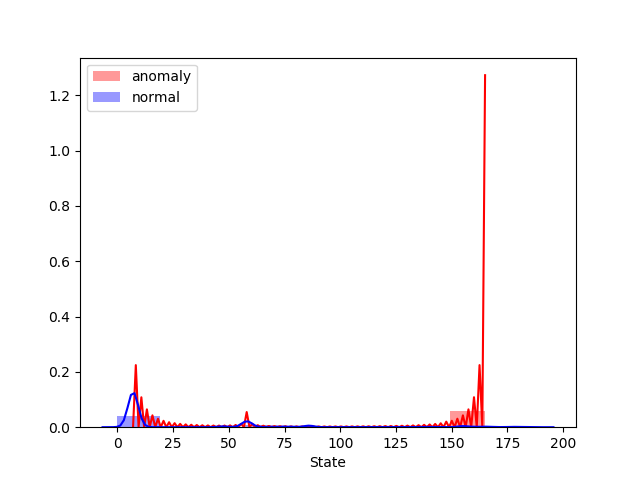
\includegraphics[width=0.47\textwidth]{figures/ch4/raw_distplot_capture20110816_State.png}
		\label{fig:4.05}
	}
	\subfigure[Destination Type of service of scenario 10.]{%
		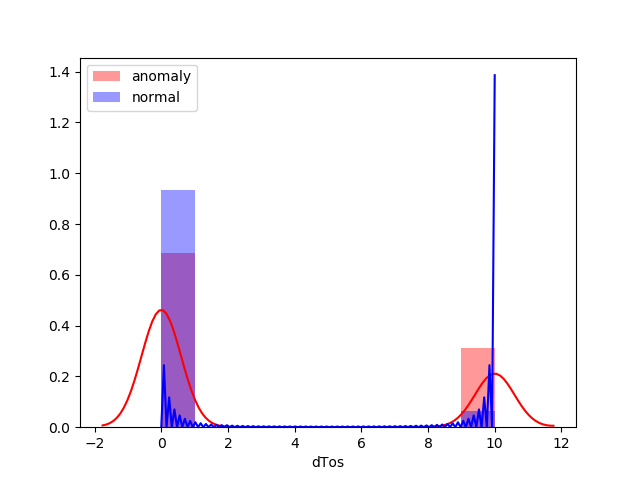
\includegraphics[width=0.47\textwidth]{figures/ch4/raw_distplot_capture20110810_dTos.png}
		\label{fig:4.06}
	}
	\caption[Skewness and Overlapping]{Example of skewness and overlapping}
	\label{fig:4.07}
\end{figure}

However, it is not possible to observe a pattern on distributions of all the features and scenarios of CTU-13, as depicted by Figures \ref{fig:4.08} and \ref{fig:4.09}, that show the distributions of TCP states of the scenario 10 and source ports of scenario 16, and highlight the distributions of normal and anomalous flows.

\begin{figure}[!htb]
	\centering
	\subfigure[State of scenario 10.]{%
		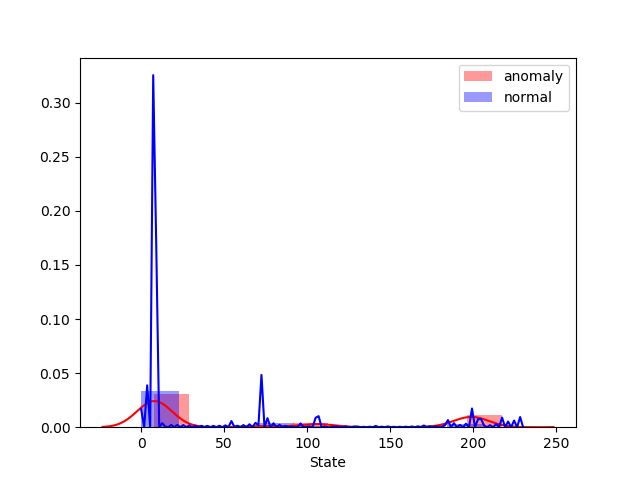
\includegraphics[width=0.47\textwidth]{figures/ch4/raw_distplot_capture20110810_State.png}
		\label{fig:4.08}
	}
	\subfigure[Source Port of scenario 16.]{%
		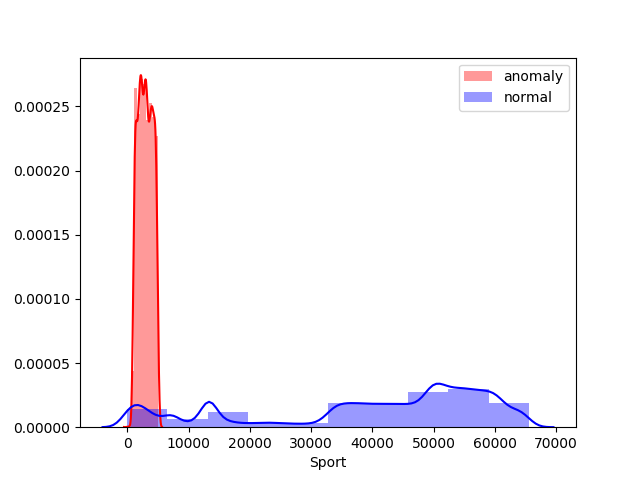
\includegraphics[width=0.47\textwidth]{figures/ch4/raw_distplot_capture20110816_Sport.png}
		\label{fig:4.09}
	}
	\caption[Skewness and Overlapping]{Skewness and Overlapping}
	\label{fig:4.10}
\end{figure}

Due to the number of available features and the class overlapping between normal and anomalous flows, we performed an correlation analysis and an empirical cross validation in order to identify the best set of features for network attack detection. Therefore, we adopt the following features: state, destination type of service, destination port, source port, total number of packets, total number of bytes and number of bytes from the source.


\section{Moment Distances from Robust Subspace for Network Attack Detection}
\label{sec:4_proposal}

This section describes the proposed approach for network attack detection by means of a distance analysis between moments computed from a robust subspace and contaminated observations of network traffic. 

Robust subspace learning can be defined as the decomposition of a given data matrix $\pmb{X}$ into the sum of a low rank matrix $\pmb{L}$, whose column subspace gives the principal components, and a sparse matrix $\pmb{S}$, with outliers or noise. We propose to learn a robust subspace $\pmb{L}$ from the normal traffic $\pmb{X}^s$ for computing $\pmb{L}^s$, $\pmb{S}^s$ and the robust moments, i.e. the mean $\bar{\pmb{x}}$, skewness $\bar{\pmb{s}}$ and kurtosis $\bar{\pmb{k}}$, in order to evaluate the distance $\pmb{d}$ between contaminated observations $\pmb{X}^c$ and moments computed from the learned robust subspace, in order to classify as anomalous the observations with the largest distances.

RPCA is a well known method to recover a low-rank matrix $\pmb{L}$ and sparse matrix $\pmb{S}$ from corrupted measurements modeled as $\pmb{X} = \pmb{L} + \pmb{S}$. This decomposition in low-rank and sparse matrices can be achieved by techniques such as Principal Component Pursuit method (PCP), and by optimization methods, such as the Augmented Lagrange Multiplier Method (ALM), Alternating Direction Method (ADM), Fast Alternating Minimization (FAM) or Iteratively Reweighted Least Squares (IRLS) \cite{candes2011robust,vaswani2018robust,lerman2018overview}.

According to Wright et al. \cite{wright2009robust}, under rather broad conditions, as long as the error matrix $\pmb{S}$ is sufficiently sparse, it is possible to recover a low-rank matrix by solving the following convex optimization problem:
\begin{equation}\label{eq:4.01}
	(\hat{\pmb{L}}, \hat{\pmb{S}})\leftarrow \min_{\pmb{L},\pmb{S}}\left \| \pmb{L} \right \|_{*} + \lambda \left \| \pmb{S} \right \|_{1}
\end{equation}
\begin{center} subject to: $\pmb{X} = \pmb{L} + \pmb{S}$ \end{center}
\begin{equation}\label{eq:4.02}
    \left \| \pmb{L} \right \|_{*} = \sum_{i} \sigma_{i}(\pmb{L})
\end{equation}
\begin{equation}\label{eq:4.03}
    \left \| \pmb{S} \right \|_{1} = \sum_{ij} \left | \pmb{S}_{ij} \right |
\end{equation}
where $\lambda$ is a positive weighting parameter, which determines the sparsity of $\pmb{S}$, $\sigma$ denotes the singular values of a matrix. 

Before ALM, some methods were proposed to solve that convex optimization problem, such as Iterative Thresholding (IT) and Accelerated Proximal Gradient (APG). However, according to Zhouchen \emph{et al.} \cite{lin2010augmented}, both approaches have scalability problems and require a large number of iterations to converge. The Augmented Lagrange Multiplier (ALM) is proven to have a \emph{Q-linear} convergence speed and experimental results show that ALM is five times faster than APG, which in theory is sub-linear \cite{lin2010augmented}. Furthermore, ALM reaches more accurate results with less iterations.

The RPCA with ALM can be formulated:
\begin{equation}\label{eq:4.04}
	l(\pmb{L}, \pmb{S}, \pmb{Y}) = \left\|\pmb{L}\right\|_* + \lambda\left\|\pmb{S}\right\|_1 + \langle \pmb{Y}, \pmb{X} - \pmb{L} - \pmb{S}  \rangle + \frac{\mu}{2}\left\|\pmb{X} - \pmb{L} - \pmb{S}\right\|_F^2,
\end{equation}
where $\pmb{Y}$ is the multiplier of the linear constraint, $\mu$ is the penalty parameter for the violation of the linear constraint \cite{yuan2009sparse}. Thus, an iterative scheme can be presented as:
\begin{equation}\label{eq:4.05}
	\left\{
		\begin{matrix} 
			(\pmb{L}_{k+1}, \pmb{S}_{k+1}) \in \operatorname*{argmin}_{\pmb{L,S} \in \mathbb{R}^{m \times n}} \{l(\pmb{L}, \pmb{S}, \pmb{Y}_{k})\}, \\ 
			\pmb{Y}_{k+1} = \pmb{Y}_{k} + \mu(\pmb{X} - \pmb{L}_{k} - \pmb{S}_{k}),
		\end{matrix}
	\right.
\end{equation}

We adopt RPCA with ADM, which, generally speaking, is a practical improvement of the classical ALM method for solving convex programming problem with linear constraints, by fully taking advantage of its high-level separable structure \cite{yuan2009sparse}. ADM minimizes $\pmb{L}$ and $\pmb{S}$ variables serially by solving the following problems to generate the new iterate:

\begin{equation}\label{eq:4.06}
	\left\{\begin{matrix}
	\pmb{L}_{k+1} \in \operatorname*{argmin}_{\pmb{L} \in \mathbb{R}^{m \times n}}\{l(\pmb{L}, \pmb{S}_{k}, \pmb{Y}_{k})\}\\ 
	\pmb{S}_{k+1} \in \operatorname*{argmin}_{\pmb{S} \in \mathbb{R}^{m \times n}}\{l(\pmb{L}_{k+1}, \pmb{S}, \pmb{Y}_{k})\}\\ 
	\pmb{Y}_{k+1} = \pmb{Y}_{k} + \mu(\pmb{X} - \pmb{L}_{k} - \pmb{S}_{k})
	\end{matrix}\right.
\end{equation}

Moments are a set of statistical parameters to measure a distribution. The arithmetic mean is the first general moment, the second is the variance, while skewness (asymmetry) is the third moment and kurtosis (excess) is the fourth moment.

Let the mean $\bar{\pmb{x}} \in \mathbb{R}^{1 \times p}$ be

\begin{equation}\label{eq:4.07}
	\bar{\pmb{x}} = \displaystyle\frac{1}{h}\displaystyle\sum_{i\in \pmb{h}} \pmb{x}_i, 
\end{equation}

and the covariance matrix $\bar{\pmb{\Sigma}} \in \mathbb{R}^{p \times p}$ be

\begin{equation}\label{eq:4.08}
	\bar{\pmb{\Sigma}} = \displaystyle\frac{1}{h}\displaystyle\sum_{i\in \pmb{h}} (\pmb{x}_i - \bar{\pmb{x}})(\pmb{x}_i - \bar{\pmb{x}})^\prime,
\end{equation}

The general formula of the $u$-th moment can be expressed as
\begin{equation}\label{eq:4.09}
	\pmb{m}_u = \displaystyle\frac{1}{n}\displaystyle\sum_{i = 1}^{n}(\pmb{x}_i - \bar{\pmb{x}})^u.
\end{equation}

Therefore, the skewness is calculated by
\begin{equation}\label{eq:4.10}
	\bar{\pmb{s}} = \frac{\pmb{m}_3}{\pmb{m}_2^{\frac{3}{2}}},
\end{equation}

and the kurtosis as
\begin{equation}\label{eq:4.11}
	\bar{\pmb{k}} = \frac{\pmb{m}_4}{\pmb{m}_2^2}.
\end{equation}

We propose to compute the mean $\bar{\pmb{x}}$, the skewness $\bar{\pmb{s}}$, the kurtosis $\bar{\pmb{k}}$ and the covariance matrix $\bar{\pmb{\Sigma}}$ from the robust subspace $\pmb{L}^s$, after to minimize the Equation \ref{eq:4.06} for $\pmb{X}^s$. We also propose to compute the Mahalanobis Distance (MD) for detecting anomalies between contaminated observations and the moments calculated from a robust subspace computed by RPCA. 

The classical Mahalanobis Distance is defined as		
\begin{equation}\label{eq:4.12}
	\pmb{d}(\pmb{x},\bar{\pmb{x}}, \bar{\pmb{\Sigma}}) = \sqrt{(\pmb{x} - \bar{\pmb{x}}) \bar{\pmb{\Sigma}}^{-1}(\pmb{x} - \bar{\pmb{x}})^\prime},
\end{equation}
where $\pmb{x}$ is a vector of a new observation, $\bar{\pmb{x}}$ is the mean vector of known observations, also referred as location, and $\bar{\pmb{\Sigma}}$ is the covariance matrix of known observations, also referred as scatter. The classical MD usually relies on robust mean and robust covariance matrix for outlier detection, which are commonly computed by MCD \cite{rousseeuw1984mcd, rousseeuw1999fastmcd}. Here we propose to calculate the MD according to Equation \ref{eq:4.12} by means of the mean and covariance matrix computed from a robust subspace learned by RPCA. 

We also propose to extend the Equation \ref{eq:4.12} to implement a Skewness-based Mahalanobis Distance, as follows:

\begin{equation}\label{eq:4.13}
	\pmb{d}(\pmb{x}, \bar{\pmb{s}}, \bar{\pmb{\Sigma}}) = \sqrt{(\pmb{x} - \bar{\pmb{s}}) \bar{\pmb{\Sigma}}^{-1}(\pmb{x} - \bar{\pmb{s}})^\prime}.
\end{equation}

Finally, we propose to extend the Equation \ref{eq:4.12} to implement a Kurtosis-based Mahalanobis Distance, as follows:

\begin{equation}\label{eq:4.14}
	\pmb{d}(\pmb{x}, \bar{\pmb{k}}, \bar{\pmb{\Sigma}}) = \sqrt{(\pmb{x} - \bar{\pmb{k}}) \bar{\pmb{\Sigma}}^{-1}(\pmb{x} - \bar{\pmb{k}})^\prime}.
\end{equation}

The distances $\pmb{d}(\pmb{x},\bar{\pmb{x}}, \bar{\pmb{\Sigma}})$, $\pmb{d}(\pmb{x}, \bar{\pmb{s}}, \bar{\pmb{\Sigma}})$ and $\pmb{d}(\pmb{x}, \bar{\pmb{k}}, \bar{\pmb{\Sigma}})$ shall be computed and evaluated separately and independently, for network attack detection. Therefore, the robust subspace learning from normal data combined to MD is called as md-RPCA when using mean-based MD, or is called sd-RPCA when using skewness-based MD, or kd-RPCA when using kurtosis-based MD.

The contamination rate parameter is widely adopted for well established outlier detection algorithms \cite{zhao2019pyod}, and refers to the percentage of observations that are classified as anomalous. The contamination rate can be well known for some areas, or can be computed by cross-validation or can be assumed according to previous observations. In our proposal, the contamination defines the number of the largest distances $\pmb{d}$ that shall be classified as anomalous. The observations classified as legitimate and anomalous, according to the contamination $c$, are denoted by the vector $\bar{\pmb{t}}$, with values of 1 for classifying anomalies and 0 to denote legitimate observation.

The Algorithm \ref{alg:4.01} describes all possible steps of m-RPCA and the approaches md-RPCA, sd-RPCA and kd-RPCA, for the semi-supervised learning approach. The unsupervised approach adopts the same steps, but adopting the contaminated data for robust subspace learning, and requiring new robust subspace learning for testing anomaly detection on new set of observations.

\begin{algorithm}
	\label{alg:4.01}
	\SetAlgoLined
	\KwResult{$\bar{\pmb{t}}_{\bar{\pmb{x}}}$, $\bar{\pmb{t}}_{\bar{\pmb{s}}}$, $\bar{\pmb{t}}_{\bar{\pmb{k}}}$}
	Given $\pmb{X}$ split into $\pmb{X}^s$ and $\pmb{X}^c$\;
	\While{not $\min_{L,S}\left \| \pmb{L} \right \|_{*} + \lambda \left \| \pmb{S} \right \|_{1}$ of $\pmb{X}^s$}{
		$\pmb{L}_{k+1} \in \operatorname*{argmin}_{\pmb{L} \in \mathbb{R}^{m \times n}}\{l(\pmb{L}, \pmb{S}_{k}, \pmb{Y}_{k})\}$\;
		$\pmb{S}_{k+1} \in \operatorname*{argmin}_{\pmb{S} \in \mathbb{R}^{m \times n}}\{l(\pmb{L}_{k+1}, \pmb{S}, \pmb{Y}_{k})\}$\;
		$\pmb{Y}_{k+1} = \pmb{Y}_{k} + \mu(\pmb{X} - \pmb{L}_{k} - \pmb{S}_{k})$\;
	}
	$\bar{\pmb{x}} = \displaystyle\frac{1}{h}\displaystyle\sum_{i\in \pmb{h}} \pmb{x}_i$, for $\pmb{L}^s$\;
	$\bar{\pmb{\Sigma}} = \displaystyle\frac{1}{h}\displaystyle\sum_{i\in \pmb{h}} (\pmb{x}_i - \bar{\pmb{x}})(\pmb{x}_i - \bar{\pmb{x}})^\prime$, for $\pmb{L}^s$\;
	$\bar{\pmb{s}} = \frac{\pmb{m}_3}{\pmb{m}_2^{\frac{3}{2}}}$, for $\pmb{L}^s$\;
	$\bar{\pmb{k}} = \frac{\pmb{m}_4}{\pmb{m}_2^2}$, for $\pmb{L}^s$\;
	$\pmb{d}(\pmb{x},\bar{\pmb{x}}, \bar{\pmb{\Sigma}}) = \sqrt{(\pmb{x} - \bar{\pmb{x}}) \bar{\pmb{\Sigma}}^{-1}(\pmb{x} - \bar{\pmb{x}})^\prime}$\;
	$\pmb{d}(\pmb{x}, \bar{\pmb{s}}, \bar{\pmb{\Sigma}}) = \sqrt{(\pmb{x} - \bar{\pmb{s}}) \bar{\pmb{\Sigma}}^{-1}(\pmb{x} - \bar{\pmb{s}})^\prime}$\;
	$\pmb{d}(\pmb{x}, \bar{\pmb{k}}, \bar{\pmb{\Sigma}}) = \sqrt{(\pmb{x} - \bar{\pmb{k}}) \bar{\pmb{\Sigma}}^{-1}(\pmb{x} - \bar{\pmb{k}})^\prime}$\;
	$\bar{\pmb{t}}_{\bar{\pmb{x}}} = [\pmb{d}(\pmb{x}, \bar{\pmb{x}}, \bar{\pmb{\Sigma}})]^c$\;
	$\bar{\pmb{t}}_{\bar{\pmb{s}}} = [\pmb{d}(\pmb{x}, \bar{\pmb{s}}, \bar{\pmb{\Sigma}})]^c$\;
	$\bar{\pmb{t}}_{\bar{\pmb{k}}} = [\pmb{d}(\pmb{x}, \bar{\pmb{k}}, \bar{\pmb{\Sigma}})]^c$\;
	\caption{Moment Distances from Robust Subspace}
\end{algorithm}

The steps between 1 and 10 of the Algorithm \ref{alg:4.01} are the training from normal data $\pmb{X}^s$, which are common steps shared by md-RPCA, sd-RPCA and kd-RPCA. The steps between 11 and 16 aim the anomaly detection from new contaminated observations, by means of Mahalanobis Distance of robust moments. Note that the steps 11 and 14 refer to the steps of md-RPCA for anomaly detection, while the steps 12 and 15 refer to the sd-RPCA, and the steps 13 and 16 refer to the steps of kd-RPCA. It is important to highlight that the anomaly detection from new observations does not require new robust subspace learning when adopting the semi-supervised approach, which only requires to compute a moment-based Mahalanobis distance to classify the $c$ largest distances as anomalous or legitimate.

The m-RPCA can also be adopted as unsupervised algorithm if the lines 1 and 2 of the Algorithm \ref{alg:4.01} are changed to substitute $\pmb{X}^s$ by $\pmb{X}^c$. Hence, the robust subspace is learned from contaminated data and used for comparing the distance between moments from robust estimate and contaminated observations. It is important to note that this unsupervised approach requires the computational cost of computing new subspace learning for any new set of observations.


\section{Experiments}
\label{sec:4_experiments}

This section presents the performed experiments on simulated and real data set for anomaly detection. First, in Section \ref{sec:4_metric} we present the adopted metric to evaluate imbalanced data in the context of anomaly detection. The Section \ref{sec:4_SimulatedScenario} describes the experiment for anomaly detection on simulated skewed and heavy-tailed data set, and the Section \ref{sec:4_CTU-13} presents the experiment for network anomaly detection on CTU-13 data set.

\subsection{The metric}
\label{sec:4_metric}

In anomalous detection problems, where anomalies are rare events, if one classify all observations as normal and apply an accuracy evaluation, one would have high accuracy but poor true-positive detection. Due to the importance given by the $F_1$ (also referred as F-score or F-measure) to true-positive detection in scenarios such as the network attack detection, it is the preferable measure for imbalanced data sets \cite{powers2011evaluation,moustafa2019holistic}. Therefore, $F_1$ is the metric used for validation of our experiments.

The $F_1$ is the harmonic mean of precision and recall and is defined by:
\begin{equation}\label{eq:4.15}
	F_1 = 2 * \frac{Precision * Recall}{Precision + Recall},
\end{equation}
where $pr$ is the precision, defined by 
\begin{equation}\label{eq:4.16}
	Precision = \frac{True Positive}{True Positive + False Positive}
\end{equation}
and $rc$ is the recall, defined by 
\begin{equation}\label{eq:4.17}
	Recall = \frac{True Positive}{True Positive + False Negative}.
\end{equation}

This experimental evaluation compares our proposal to widely adopted algorithms for anomaly detection that also rely on contamination rate for anomaly detection, which are: A PCA approach based on the sum of weighted projected distances to the eigenvector hyperplanes \cite{shyu2003novel}; MCD \cite{rousseeuw1984mcd,rousseeuw1999fastmcd}; One-Class Support Vector Machines \cite{scholkopf2001estimating}; Local Outlier Factor (LOF) \cite{breunig2000lof}; k-Nearest Neighbors \cite{angiulli2002fast}; and Isolation Forest \cite{liu2008isolation}.

We also compare the results of our proposals to ROBPCA for anomaly detection on simulated and CTU-13 data sets, considering that ROBPCA also relies on robust estimates with adjusted outlyingness based on robust skewness \cite{hubert2009robustskewed}.

\subsection{Simulated Experiment}
\label{sec:4_SimulatedScenario}

Anomaly detection algorithms usually rely on supervised or unsupervised methods, where the former requires labeled normal and anomalous data for training anomaly detection models, while the latter does not require labeled data or training. Semi-supervised algorithms are an alternative for the anomaly detection problem, considering that this method only relies on normal data for training and that non-malicious data can be obtained from historical information and from rule-based approaches. 

We propose semi-supervised and unsupervised approaches for m-RPCA, where the former relies on normal data $\pmb{X}^s$ for training and on contamination rate $c$ for anomaly detection, while the latter relies only on contaminated data $\pmb{X}^c$ for robust subspace learning and rely on contamination rate $c$ to select the largest distances. We assume that $c$ is well known or can be estimated for real world problems of anomaly detection, in accordance to the assumption adopted by the well established algorithms \cite{zhao2019pyod} selected for comparison, that also rely on contamination rate $\pmb{X}^c$.

The availability of labeled data is a challenging concern in real world problems of anomalous detection, where anomalies are rare or even unknown events. Considering that RPCA has already been adopted to isolate outliers from training data \cite{zhou2017anomaly}, we also propose to evaluate the m-RPCA for a contaminated semi-supervised approach based on training from contaminated data, in order to evaluate the impact that contaminated data for robust subspace learning can cause in the anomaly detection results.

Therefore, we propose to evaluate the following approaches for m-RPCA: semi-supervised; contaminated semi-supervised; and unsupervised.

For the semi-supervised approach we propose to learn the robust subspace and compute the moments from the normal data set $\pmb{Y}_g$, $\pmb{Y}_p$ and $\pmb{Y}_l$ with Gaussian, Pareto and Lognormal distributions, respectively, and test the anomaly detection for contaminated data set $\pmb{Y}_g^c$, $\pmb{Y}_p^c$ and $\pmb{Y}_l^c$.

For the Contaminated Semi-supervised approach we evaluate the robustness of the m-RPCA approaches for learning from contaminated training data, in order to analyse if m-RPCA can be an alternative for the lack of known normal data. Therefore we propose to train the model from a contaminated normal data $\pmb{Y}_g^{c'}$, $\pmb{Y}_p^{c'}$ and $\pmb{Y}_l^{c'}$, with the same contamination rate of the testing data, but without data repetition between training and testing, taking into account that we shall consider a different contaminated data but adopt the same contamination rate for training and testing.

We finally evaluate the unsupervised approach, that relies on the test data sets $\pmb{Y}_g^c$, $\pmb{Y}_p^c$ and $\pmb{Y}_l^c$ for robust subspace learning, and then classify the results according to the distance between the contaminated data $\pmb{Y}_g^c$, $\pmb{Y}_p^c$ and $\pmb{Y}_l^c$, and the moments computed from the learned robust subspace.

\subsection{Experiment for CTU-13}
\label{sec:4_CTU13Scenario}

In contrast to Garcia \emph{et al.} \cite{garcia2014empirical}, we propose to evaluate each scenario of the CTU-13 data set individually, in a semi-supervised approach that does not rely on training data with labeled anomalies, in order to evaluate our proposed approaches to all botnet malwares of the CTU-13 data set. 

In our experiment setup each contaminated scenario $\pmb{X}_i$ of CTU-13 is split into $\pmb{X}_i^s$, containing 50\% of the the normal data, and into test data $\pmb{X}_i^c$ containing 33\% of normal and 67\% of anomalous data. We adopt a contamination rate $c$ of 33\% for  experimenting anomaly detection for the CTU-13 data set, considering that this contamination rate presented good results on the simulated experiment for our proposals and for some selected algorithms.

This experiment consider only the semi-supervised approach due to results of simulated experiments on simulated data set presented in Subsection \ref{sec:4_simulated_result}, that shows better results for the semi-supervised approach and highlight that the this approach can obtain good results even when trained with contaminated data set.


\section{Results of Simulated Experiment}
\label{sec:4_simulated_result}

We adopt prefixes to denote the evaluated approaches for md-RPCA, sd-RPCA and kd-RPCA, which are ss\_ to denote semi-supervised, css\_ to denote contaminated semi-supervised and u\_ for unsupervised.

We initially evaluated the $F_1$ of the selected algorithms and m-RPCA approaches for anomaly detection on Gaussian distributed legitimate data contaminated by uniform distributed anomalies. The Figure \ref{fig:4.10} shows the $F_1$ over the contamination rate between 1\% and 50\% for m-RPCA approaches and Isolation Forest (IF) \cite{liu2008isolation}, k-Nearest Neighbors (KNN) \cite{angiulli2002fast}, Local Outlier Factor (LOF) \cite{breunig2000lof}, Minimum Covariance Deteminant (MCD) \cite{rousseeuw1999fastmcd}, One-Class Support Vector Machines (OCSVM) \cite{scholkopf2001estimating}, PCA \cite{shyu2003novel} and ROBPCA-AO \cite{hubert2009robustskewed}.

\begin{figure}[h!]
	\centering
	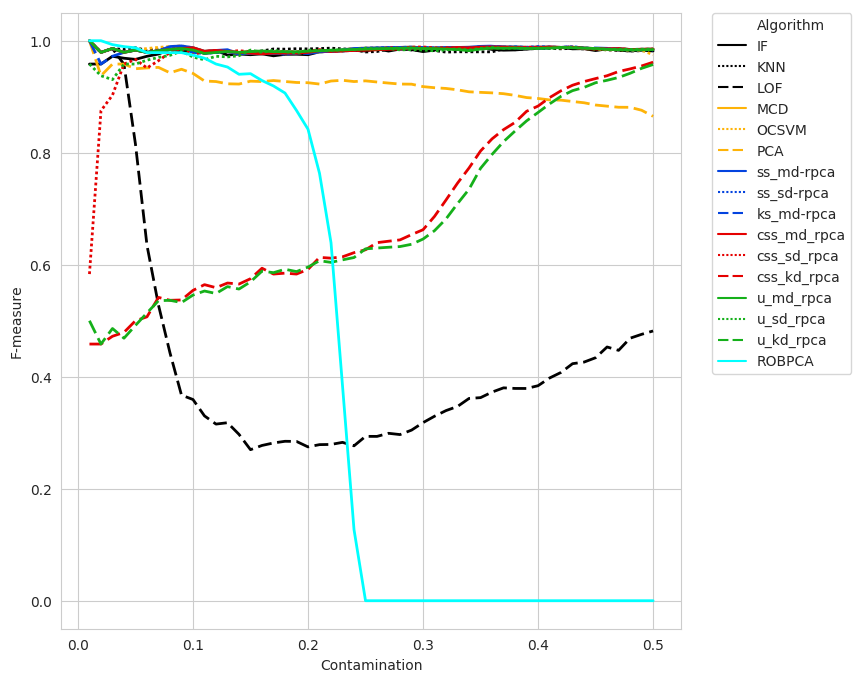
\includegraphics[width=10cm]{figures/ch4/gaussian_f1_contamination.png}
	\caption{Anomaly detection on Gaussian distributed with uniform anomalies}
	\label{fig:4.10}
\end{figure}

It is possible to observe in Figure \ref{fig:4.10} that LOF, PCA, css\_kd-RPCA and u\_kd-RPCA presented lower performance than the remain algorithms, that obtain results higher than 0.95 in average. The exception is the ROBPCA-AO, that presented high score for lower contamination but decreased with the contamination increasing. 

Note that the css\_kd-RPCA and u\_kd-RPCA are the contaminated semi-supervised and unsupervised versions of kd-RPCA, that obtain worse results than the semi-supervised approach of kd-RPCA, for anomaly detection on Gaussian distributed data contaminated by uniform anomalies. However, the unsupervised versions of md-RPCA and sd-RPCA presented similar results to widely adopted unsupervised algorithms for outlier detection. The results also show that the semi-supervised approach of md-RPCA, sd-RPCA and kd-RPCA obtain high anomaly detection rate and presented similar results to the unsupervised algorithms IF, KNN, MCD and OCSVM. 

The Figure \ref{fig:4.11} and \ref{fig:4.12} show the results for anomaly detection on skewed and heavy tailed distributions. The Figure \ref{fig:4.11} shows the results for Pareto with Gaussian anomalies.

\begin{figure}[h!]
	\centering
	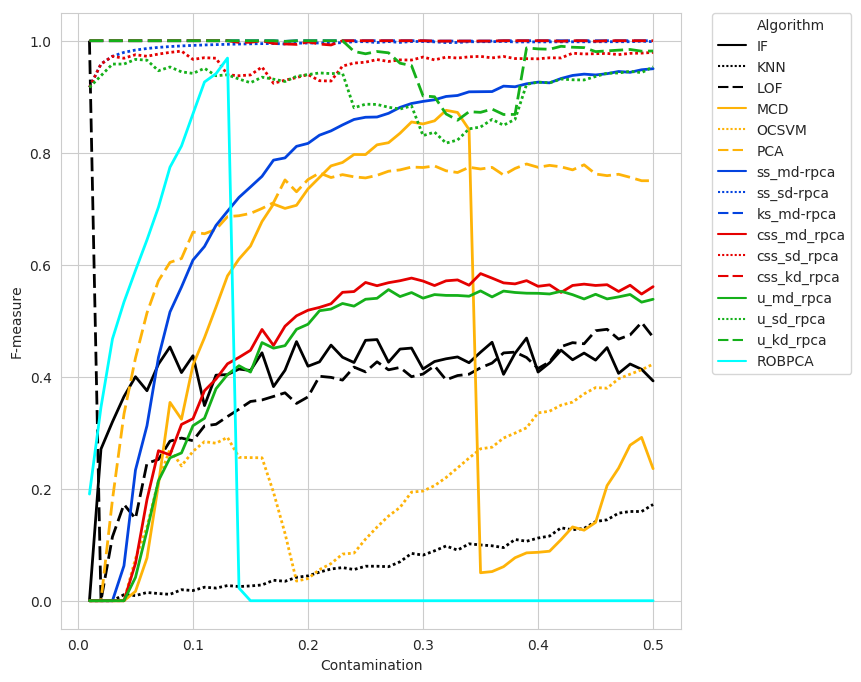
\includegraphics[width=10cm]{figures/ch4/pareto_f1_contamination.png}
	\caption{Anomaly detection on Pareto distributed with Gaussian anomalies}
	\label{fig:4.11}
\end{figure}

The results for anomaly detection on Pareto with Gaussian anomalies, depicted by Figure \ref{fig:4.11}, show that IF, KNN, LOF, OCSVM, css\_md-RPCA and u\_md-RPCA performed worse than the remain algorithms for the evaluated contamination, with results lower than 0.6 even with higher contamination. Note that the approaches of m-RPCA with lower scores are css\_md-RPCA and u\_md-RPCA, which are mean-based approaches. However, the ss\_md-RPCA is the mean-based approach that presented lower results for lower contamination but achieved more than 0.8 with contamination near of 0.2 or higher, and achieved results better than MCD and PCA.

Figure \ref{fig:4.11} shows that ROBPCA-AO presented high scores for low contamination rates, presenting results better than ss\_md-RPCA, MCD and PCA, initially. However, the results of ROBPCA-AO decrease drastically with the contamination increasing.

It is possible to observe in Figure \ref{fig:4.11} that all approaches based on kd-RPCA achieved the best results initially, but the results for the unsupervised variate with contamination near of 0.2 or higher, while the ss\_kd-RPCA presents stable results near of 1.0 $F_1$ for all evaluated contamination rates.

All approaches based on sd-RPCA obtained anomaly detection higher than 0.8, however the unsupervised and contaminated semi-supervised presented high variation of $F_1$ and lower results in comparison to the semi-supervised sd-RPCA. The contaminated semi-supervised approaches of sd-RPCA and kd-RPCA presented results higher than 0.8 and similar to the semi-supervised and unsupervised approaches of sd-RPCA and kd-RPCA. These results highlight the resilience of the robust subspace learning even for contaminated training data.

The unsupervised approaches of sd-RPCA and kd-RPCA presented more than 0.8 for all contamination rate, showing better results than the widely adopted unsupervised algorithms for outlier detection. However, u\_kd-RPCA and u\_sd-RPCA presented lower results than ss\_kd-RPCA and ss\_sd-RPCA. Therefore, the semi-supervised approaches of m-RPCA overcome other approaches of m-RPCA and overcome the selected algorithms for anomaly detection on Pareto distributed data with Gaussian anomalies. It is possible to highlight the semi-supervised kd-RPCA, which obtained stable results near of 1.0 $F_1$ for all evaluated contamination.

The results for anomaly detection on Lognormal with Gaussian anomalies, depicted by Figure \ref{fig:4.12}, show that IF, KNN, LOF, MCD, OCSVM, css\_md-RPCA, u\_md-RPCA and ROBPCA-AO perform worse than the remain evaluated algorithms, with results lower than 0.6 even with higher contamination. 

\begin{figure}[h!]
	\centering
	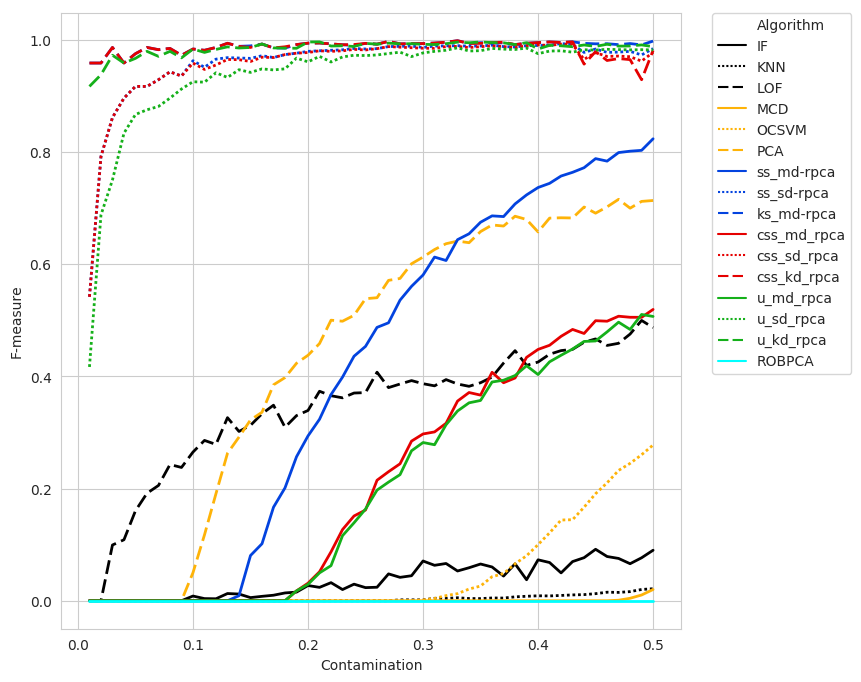
\includegraphics[width=10cm]{figures/ch4/lognormal_f1_contamination.png}
	\caption{Anomaly detection on Lognormal distributed with Gaussian anomalies}
	\label{fig:4.12}
\end{figure}

The ss\_md-RPCA and PCA algorithms perform similar, with worse detection rate for lower contamination and better performance with contamination higher than 0.4. However, the results of ss\_md-RPCA and PCA are lower than all approaches of sd-RPCA and kd-RPCA. It is important to note that all mean-based approaches of m-RPCA presented lower results for anomaly detection on Lognormal data, in comparison to approaches based on skewness (sd-RPCA) and kurtosis (kd-RPCA), that achieved the best anomaly detection rates. However, the approaches of md-RPCA presented better results than IF, KNN, MCD, OCSVM and ROBPCA-AO.

The approaches based on kd-RPCA presented higher detection rate for all contamination, with scores near of 1.0. The semi-supervised and contaminated semi-supervised approaches for sd-RPCA performed similarly, but the unsupervised approach of sd-RPCA presented lower anomaly detection for lower contamination.

It is possible to note that the contaminated semi-supervised approaches of kd-RPCA and sd-RPCA performed similar to the semi-supervised approach of the same algorithms. These results highlight the resilience of the robust subspace learning even from contaminated training data for anomaly detection on Lognormal data.

Therefore, it is possible to observe that the semi-supervised approaches of m-RPCA overcome other approaches of m-RPCA and all the selected algorithms for anomaly detection on Lognormal distributed data with Gaussian anomalies.

Following we present the Tables \ref{tab:4.02}, \ref{tab:4.03} and \ref{tab:4.04} to show the results of the selected algorithms and of our proposals for anomaly detection on Gaussian, Pareto and Lognormal distributions, with 10\%, 25\% and 33\% of contamination rate.

\begin{table}[h!]
    \centering
	\scriptsize
	\caption{Results for Simulated data set with 33\% of contamination}
	\label{tab:4.02}
	\begin{tabular}{| l | l | l | l |}
		\hline \rowcolor{Gray} \begin{tabular}[x]{@{}c@{}}\pmb{Algorithm}\end{tabular}	&\begin{tabular}[x]{@{}c@{}}\pmb{Gaussian + Uniform}\\\pmb{($F_1$)}\end{tabular}	&\begin{tabular}[x]{@{}c@{}}\pmb{Pareto + Gaussian}\\\pmb{($F_1$)}\end{tabular}	 &\begin{tabular}[x]{@{}c@{}}\pmb{Lognormal + Gaussian}\\\pmb{($F_1$)}\end{tabular}\\ \hline
            Isolation Forest	&0.98	&0.44	&0.05\\ \hline
            KNN	&0.98	&0.08	&0.00\\ \hline
            LOF	&0.35	&0.40	&0.36\\ \hline
            MCD	&0.98	&0.02	&0.00\\ \hline
            One-class SVM	&0.98	&0.24	&0.00\\ \hline
            PCA	&0.87	&0.76	&0.62\\ \hline
            Semi-Supervised md-RPCA	&0.98	&0.90	&0.66\\ \hline
            Semi-Supervised sd-RPCA	&0.98	&0.99	&0.97\\ \hline
            Semi-Supervised kd-RPCA	&0.97	&0.99	&0.98\\ \hline
            Contaminated Semi-Supervised md-RPCA	&0.98	&0.55	&0.35\\ \hline
            Contaminated Semi-Supervised sd-RPCA	&0.98	&0.94	&0.96\\ \hline
            Contaminated Semi-Supervised kd-RPCA	&0.76	&0.99	&0.98\\ \hline
            Unsupervised md-RPCA	&0.98	&0.54	&0.31\\ \hline
            Unsupervised sd-RPCA	&0.98	&0.82	&0.93\\ \hline
            Unsupervised kd-RPCA	&0.74	&0.86	&0.99\\ \hline
            ROBPCA-AO   &0.00	&0.00	&0.00\\ \hline
	\end{tabular}
\end{table}

The results with 33\% of contamination shows high scores of anomaly detection for Gaussian data with uniform anomalies, with exception to LOF and ROBPCA-AO. The semi-supervised approaches of m-RPCA presented the highest results for anomaly detection on Pareto data with Gaussian anomalies, and for anomaly detection on Lognormal data with Gaussian anomalies.

\begin{table}[h!]
    \centering
	\scriptsize
	\caption{Results for Simulated data set with 25\% of contamination}
	\label{tab:4.03}
	\begin{tabular}{| l | l | l | l |}
		\hline \rowcolor{Gray} \begin{tabular}[x]{@{}c@{}}\pmb{Algorithm}\end{tabular}	&\begin{tabular}[x]{@{}c@{}}\pmb{Gaussian + Uniform}\\\pmb{($F_1$)}\end{tabular}	&\begin{tabular}[x]{@{}c@{}}\pmb{Pareto + Gaussian}\\\pmb{($F_1$)}\end{tabular}	 &\begin{tabular}[x]{@{}c@{}}\pmb{Lognormal + Gaussian}\\\pmb{($F_1$)}\end{tabular}\\ \hline
            Isolation Forest	&0.97	&0.46	&0.05\\ \hline
            KNN	&0.97	&0.05	&0.00\\ \hline
            LOF	&0.27	&0.33	&0.30\\ \hline
            MCD	&0.97	&0.79	&0.00\\ \hline
            One-class SVM	&0.97	&0.11	&0.00\\ \hline
            PCA	&0.91	&0.75	&0.56\\ \hline
            Semi-Supervised md-RPCA	&0.97	&0.85	&0.49\\ \hline
            Semi-Supervised sd-RPCA	&0.97	&0.99	&0.96\\ \hline
            Semi-Supervised kd-RPCA	&0.96	&1.00	&0.98\\ \hline
            Contaminated Semi-Supervised md-RPCA	&0.97	&0.54	&0.17\\ \hline
            Contaminated Semi-Supervised sd-RPCA	&0.97	&0.91	&0.95\\ \hline
            Contaminated Semi-Supervised kd-RPCA	&0.63	&1.00	&0.97\\ \hline
            Unsupervised md-RPCA	&0.97	&0.53	&0.14\\ \hline
            Unsupervised sd-RPCA	&0.97	&0.88	&0.91\\ \hline
            Unsupervised kd-RPCA	&0.62	&0.97	&0.99\\ \hline
            ROBPCA-AO	&0.00	&0.00	&0.00\\ \hline
	\end{tabular}
\end{table}

The Table \ref{tab:4.03} also shows higher scores of semi-supervised m-RPCA for 25\% of contamination, in comparison to the remain algorithms. It is important to note that the highest score for anomaly detection on Lognormal data with Gaussian contamination was the unsupervised kd-RPCA, and that the contaminated semi-supervised approaches presented scores near of the the results for semi-supervised approaches.

\begin{table}[h!]
    \centering
	\scriptsize
	\caption{Results for Simulated data set with 10\% of contamination}
	\label{tab:4.04}
	\begin{tabular}{| l | l | l | l |}
		\hline \rowcolor{Gray} \begin{tabular}[x]{@{}c@{}}\pmb{Algorithm}\end{tabular}	&\begin{tabular}[x]{@{}c@{}}\pmb{Gaussian + Uniform}\\\pmb{($F_1$)}\end{tabular}	&\begin{tabular}[x]{@{}c@{}}\pmb{Pareto + Gaussian}\\\pmb{($F_1$)}\end{tabular}	 &\begin{tabular}[x]{@{}c@{}}\pmb{Lognormal + Gaussian}\\\pmb{($F_1$)}\end{tabular}\\ \hline
            Isolation Forest	&0.97	&0.43	&0.00\\ \hline
            KNN	&0.97	&0.01	&0.00\\ \hline
            LOF	&0.29	&0.27	&0.24\\ \hline
            MCD	&0.97	&0.40	&0.00\\ \hline
            One-class SVM	&0.97	&0.26	&0.00\\ \hline
            PCA	&0.92	&0.65	&0.06\\ \hline
            Semi-Supervised md-RPCA	&0.97	&0.59	&0.00\\ \hline
            Semi-Supervised sd-RPCA	&0.97	&0.98	&0.84\\ \hline
            Semi-Supervised kd-RPCA	&0.97	&1.00	&0.95\\ \hline
            Contaminated Semi-Supervised md-RPCA	&0.97	&0.28	&0.00\\ \hline
            Contaminated Semi-Supervised sd-RPCA	&0.96	&0.90	&0.82\\ \hline
            Contaminated Semi-Supervised kd-RPCA	&0.48	&1.00	&0.94\\ \hline
            Unsupervised md-RPCA	&0.97	&0.31	&0.00\\ \hline
            Unsupervised sd-RPCA	&0.97	&0.93	&0.70\\ \hline
            Unsupervised kd-RPCA	&0.50	&0.97	&0.98\\ \hline
            ROBPCA-AO	&0.97	&0.87	&0.00\\ \hline
	\end{tabular}
\end{table}

The contamination rate of 10\% shown by Table \ref{tab:4.03} shows worse results in comparison to contamination of 25\% and 33\%. However, the ROBPCA-AO presented high scores for anomaly detection on Gaussian data, overcoming LOF, css\_kd-RPCA and u\_kd-RPCA. ROBPCA also presented better results for anomaly detection on Pareto data in comparison to u\_md-RPCA, css\_md-RCAP, ss\_md-RCAP, PCA, OCSVM, LOF, KNN and IF.

Taking into account the null hypothesis $H_{0rob.sub}$ and the presented results, we can conclude that the robust subspace learning, adopted by md-RPCA, sd-RPCA and kd-RPCA, presented higher anomaly detection from imbalanced and skewed data than widely adopted algorithms for anomaly detection. Therefore, the presented results refute the null hypothesis $H_{0rob.sub}$, which defines that the robust subspace learning does not improves the anomaly detection from imbalanced and skewed data.

\section{Results of CTU-13 Experiment}
\label{sec:4_ctu13_result}

In this section we present the experiment on network anomaly detection from the CTU-13 data set, evaluating the results of md-RPCA, sd-RPCA, kd-RPCA, Isolation Forest (IF) \cite{liu2008isolation}, k-Nearest Neighbors (KNN) \cite{angiulli2002fast}, Local Outlier Factor (LOF) \cite{breunig2000lof}, Minimum Covariance Deteminant (MCD) \cite{rousseeuw1999fastmcd}, One-Class Support Vector Machines (OCSVM) \cite{scholkopf2001estimating}, PCA \cite{shyu2003novel} and ROBPCA-AO \cite{hubert2009robustskewed}.

For this experiment we only evaluate the semi-supervised approach of md-RPCA, sd-RPCA and kd-RPCA, considering that the semi-supervised algorithms presented the best results on the simulated experiment and taking into account the observed resilience of the semi-supervised approach when the training data is contaminated. Additionally, the semi-supervised approach only requires the robust subspace learning for training, what can indicate less computational cost for network anomaly detection on new observations.

The CTU-13 data set is very imbalanced, with contamination rate between 0.06\% and 8.86\%. Therefore we adopted a uniform contamination rate of 33\% for this experiment, considering that the simulated experiment showed better results for contamination higher than 30\% for m-RPCA and for the selected anomaly detection algorithms.

\begin{table}[h!]
  \centering
  \scriptsize
  \caption{Network anomaly detection from CTU-13 with 33\% of contamination}
  \label{tab:4.05}
  \begin{tabular}{ c|c|c|c|c|c|c|c|c|c|c|c|c|c|c }
	\toprule
        \pmb{Algorithm}	&\pmb{10}	&\pmb{11}	&\pmb{12}	&\pmb{15}	&\pmb{15-2}	&\pmb{15-3}	&\pmb{16}	&\pmb{16-2}	&\pmb{16-3}	&\pmb{17}	&\pmb{18}	&\pmb{18-2}	&\pmb{19}	&\pmb{Avg} \\ \hline
        IF	&0.36	&0.34	&0.09	&0.21	&0.40	&0.44	&0.16	&0.34	&0.34	&0.41	&0.12	&0.16	&0.46	&0.29\\ \hline
        KNN	&0.05	&0.17	&0.01	&0.03	&0.33	&0.23	&0.01	&0.25	&0.03	&0.12	&0.00	&0.00	&0.24	&0.11\\ \hline
        LOF	&0.15	&0.14	&0.13	&0.17	&0.29	&0.22	&0.29	&0.38	&0.25	&0.24	&0.00	&0.04	&0.38	&0.21\\ \hline
        MCD	&0.18	&0.29	&0.09	&0.34	&0.79	&0.62	&0.04	&0.58	&0.20	&0.41	&0.20	&0.20	&0.36	&0.33\\ \hline
        PCA	&0.33	&0.64	&0.69	&0.65	&0.55	&0.62	&0.75	&0.50	&0.77	&0.33	&0.82	&0.01	&0.61	&0.56\\ \hline
        md-RPCA &0.83	&0.79	&0.95	&0.78	&0.78	&0.87	&0.95	&0.87	&0.80	&0.82	&0.83	&0.82	&0.51	&0.81\\ \hline
        sd-RPCA &0.25	&0.75	&0.34	&0.64	&0.50	&0.75	&0.86	&0.50	&0.77	&0.33	&0.82	&0.81	&0.21	&0.57\\ \hline
        kd-RPCA &0.76	&0.76	&0.90	&0.82	&0.57	&0.76	&0.91	&0.50	&0.80	&0.73	&0.83	&0.81	&0.48	&0.74\\ \hline
        ROBPCA-AO &0.01	&0.07	&0.00	&0.05	&0.38	&0.11	&0.05	&0.32	&0.03	&0.09	&0.07	&0.09	&0.21	&0.11\\ \hline
    \bottomrule
  \end{tabular}
\end{table}

The Table \ref{tab:4.03} present the $F_1$ of each algorithm for all scenarios of CTU-13, and the last column presents the average $F_1$ of each algorithm for all scenarios.

It is possible to observe that md-RPCA, kd-RPCA and sd-RPCA overcome the remain algorithms in average results for all scenarios, according to the column \pmb{avg}. The sd-PRCA presented an average of 0.57 while md-RPCA obtained 0.81 and kd-RPCA 0.74 in average. The PCA algorithm performed similar to sd-RPCA in average, with results of 0.56 and 0.57, respectively. However the results of PCA and sd-RPCA for scenarios 12, 18-2 and 19 presented a large variation.

The md-RPCA algorithm presented an anomaly detection rate higher than 0.78 for almost all scenarios, with exception to scenario 19, where the anomaly detection rate of md-RPCA was 0.51. The anomalies of the scenario 19 are peer-to-peer botnet traffic generated by nsys.ay, which are related to botnet synchronization and not to network attacks, what can explain the low network detection rate of all evaluated algorithms, where the largest $F_1$ was 0.61 achieved by PCA.

The md-RPCA showed the best anomaly detection for 10 scenarios of a total with 13 scenarios. In the scenario 15 the best result was obtained by kd-RPCA, for the 15-2 scenario the best result was for MCD, and PCA was the best algorithm for scenario 19. Even thought md-RPCA not be the best result for scenarios 15, 15-2 and 19, the results of md-RPCA are very close to the best results for scenarios 15 and 15-2.

It is important to note that IF, KNN, LOF, MCD and ROBPCA-AO present the worse results for network attack detection on all scenarios of the CTU-13 data set, with average of 0.29, 0.11, 0.21, 0.33 and 0.11 respectively. From these algorithms, only MCD presented high result for one scenario, which was 0.79 for 15-2.

The CTU-13 data set is very challenging for anomaly detection approaches, due to the high imbalance and large volume of flows. However, CTU-13 is one of the up-to-date data sets for network attack detection and is one that provides the data imbalance observed in real anomaly detection problems. Unfortunately, was not possible to observe Pareto or Lognormal distributions on features of CTU-13, even though the finds of researches that highlight the fitting between these distributions and Internet traffic \cite{benson2010network, leon2017probability}. 

The results of anomaly detection on CTU-13 reveals that m-RPCA algorithms obtain good results for network attack detection on contaminated data, overcoming widely adopted algorithms for outlier detection.


\section{Conclusion}
\label{sec:4_conclusion}

This work proposed the m-RPCA, which is approaches based on distances of moments computed from a robust subspace learned by RPCA, for anomaly detection on imbalanced and skewed data. We evaluated the anomaly detection rate of m-RPCA for simulated data and for the CTU-13 data set, which is composed by network traffic of botnets, attacks and background flows.

The m-RPCA can be divided into md-RPCA, sd-RPCA and kd-RPCA algorithms, to denote approaches of m-RPCA based on distances of mean, skewness and kurtosis, respectively. We also proposed to evaluate m-RPCA for semi-supervised, contaminated semi-supervised and unsupervised methods of anomaly detection.

The experimental results show that moment distances computed from robust subspace can improve the anomaly detection on skewed and imbalanced data set. The results also show that the m-RPCA can be adopted for network attack detection, with better results than widely adopted algorithms for outlier detection on the CTU-13 data set. Therefore, the observed results rejects the null hypothesis  $H_{0rob.sub}$ and confirms the alternative
hypothesis $H_{1rob.sub}$.

The results shows that the semi-supervised approach for m-RPCA obtained better results than the contaminated semi-supervised and unsupervised approaches, and that m-RPCA presented good results even when the semi-supervised training was computed from contaminated data. This highlights the resilience of the robust subspace learning for the semi-supervised anomaly detection approach to deal with possible lack of known normal data for training. 

The main contributions of this work were: the development and evaluation of novel approaches for anomaly detection on skewed and imbalanced data sets, by means of moments computed from a robust subspace learned by RPCA; the evaluation of the proposed approaches for anomaly detection on simulated data set and for network attack detection on real botnet traffic data set. 

Future research can be directed to evaluate the application of the proposed approaches to different data sets and anomaly detection problems. The m-RPCA can also be extended to be online and to learn new subspace in a adaptive fashion, by means of new robust subspace learning from new observations or through robust subspace tracking.